% --- Template for thesis / report with tktltiki2 class ---
%
% last updated 2013/02/15 for tkltiki2 v1.02

\documentclass[finnish]{tktltiki2}

  % tktltiki2 automatically loads babel, so you can simply
  % give the language parameter (e.g. finnish, swedish, english, british) as
  % a parameter for the class: \documentclass[finnish]{tktltiki2}.
  % The information on title and abstract is generated automatically depending on
  % the language, see below if you need to change any of these manually.
  %
  % Class options:
  % - grading                 -- Print labels for grading information on the front page.
  % - disablelastpagecounter  -- Disables the automatic generation of page number information
  %                              in the abstract. See also \numberofpagesinformation{} command below.
  %
  % The class also respects the following options of article class:
  %   10pt, 11pt, 12pt, final, draft, oneside, twoside,
  %   openright, openany, onecolumn, twocolumn, leqno, fleqn
  %
  % The default font size is 11pt. The paper size used is A4, other sizes are not supported.
  %
  % rubber: module pdftex

  % --- General packages ---

  \usepackage[utf8]{inputenc}
  \usepackage[T1]{fontenc}
  \usepackage{lmodern}
  \usepackage{microtype}
  \usepackage{amsfonts,amsmath,amssymb,amsthm,booktabs,color,enumitem,graphicx}
  \usepackage[pdftex,hidelinks]{hyperref}

  \graphicspath{{images/}}

  % Automaticall set the PDF metadata fields
  \makeatletter
  \AtBeginDocument{\hypersetup{pdftitle = {\@title}, pdfauthor = {\@author}}}
  \makeatother

  % --- Language-related settings ---
  %
  % these should be modified according to your language

  % babelbib for non-english bibliography using bibtex
  \usepackage[fixlanguage]{babelbib}
  \selectbiblanguage{finnish}

  % add bibliography to the table of contents
  \usepackage[nottoc]{tocbibind}
  % tocbibind renames the bibliography, use the following to change it back
  \settocbibname{Lähteet}

  % --- Theorem environment definitions ---

  \newtheorem{lau}{Lause}
  \newtheorem{lem}[lau]{Lemma}
  \newtheorem{kor}[lau]{Korollaari}

  \theoremstyle{definition}
  \newtheorem{maar}[lau]{Määritelmä}
  \newtheorem{ong}{Ongelma}
  \newtheorem{alg}[lau]{Algoritmi}
  \newtheorem{esim}[lau]{Esimerkki}

  \theoremstyle{remark}
  \newtheorem*{huom}{Huomautus}


  % --- tktltiki2 options ---
  %
  % The following commands define the information used to generate title and
  % abstract pages. The following entries should be always specified:

  \title{Konvolutionaaliset neuroverkot}
  \author{Teemu Sarapisto}
  \date{\today}
  \level{Kandidaatintutkielma}
  \abstract{
  Viimeisen hieman yli kymmenen vuoden aikana voidaan sanoa keinotekoisten neuroverkkojen ja syväoppimisen tehneen läpimurron. Syväoppimisen voidaan katsoa syntyneen jo 40-luvulla, mutta laajamittaiseen sovelluskäyttöön se on tullut vasta viime vuosina, kun sekä riittävä määrä luokiteltua dataa, että riittävästi prosessointitehoa on tullut helposti saataville. Myös algoritmipuolella tapahtuneet edistykset ovat edesauttaneet läpimurtoa. Aikaisemmin koneoppimisen alalla haasteelliseksi osoittautuneissa sovelluskohteissa kuten kuvien sekä puheen sisällön tunnistamisessa keinotekoiset neuroverkot ovat osoittautuneet toistaiseksi ylivoimaisesti parhaiten toimiviksi ratkaisuiksi.
  
  Neuroverkkojen opetuksessa tärkeimpiä menetelmiä ovat gradienttimenetelmä ja takaisinvirtausalgoritmi
  
  Konvolutionaaliset neuroverkot ovat eräänlaisia neuroverkkoja jotka soveltuvat hyvin kuvien ja muiden paikallisuudesta hyötyvien syötteiden käsittelyyn}

  % The following can be used to specify keywords and classification of the paper:

  \keywords{neuroverkot, neuroverkkojen harjoittaminen, konvolutionaaliset neuroverkot, kuvien luokittelu}

  % classification according to ACM Computing Classification System (http://www.acm.org/about/class/)
  % This is probably mostly relevant for computer scientists
  % uncomment the following; contents of \classification will be printed under the abstract with a title
  % "ACM Computing Classification System (CCS):"
  % \classification{}

  % If the automatic page number counting is not working as desired in your case,
  % uncomment the following to manually set the number of pages displayed in the abstract page:
  %
  % \numberofpagesinformation{16 sivua + 10 sivua liitteissä}
  %
  % If you are not a computer scientist, you will want to uncomment the following by hand and specify
  % your department, faculty and subject by hand:
  %
  % \faculty{Matemaattis-luonnontieteellinen}
  % \department{Tietojenkäsittelytieteen laitos}
  % \subject{Tietojenkäsittelytiede}
  %
  % If you are not from the University of Helsinki, then you will most likely want to set these also:
  %
  % \university{Helsingin Yliopisto}
  % \universitylong{HELSINGIN YLIOPISTO --- HELSINGFORS UNIVERSITET --- UNIVERSITY OF HELSINKI} % displayed on the top of the abstract page
  % \city{Helsinki}
  %


  \begin{document}

  % --- Front matter ---

  \frontmatter      % roman page numbering for front matter

  \maketitle        % title page
  \makeabstract     % abstract page

  \tableofcontents  % table of contents

  % --- Main matter ---

  \mainmatter       % clear page, start arabic page numbering

  \section{Johdanto}
   Syväoppimisen historia ulottuu 1940-luvulle asti \cite{Goodfellow-et-al-2016}, jolloin kybernetiikan tutkimuksen myötä McCulloch ja Pitts kehittivät mukaansa nimetyn McCulloch-Pitts neuronin, tarkoituksenaan luoda matemaattinen malli, jolla kuvailla biologista aivoissa tapahtuvaa oppimista \cite{mcculloch1943logical}. Heidän kehittelemällään lineaarisella mallilla oli mahdollista tunnistaa kahden syötekategorian välillä kategoriat määrittelevien painotuksien avulla ihmisen joutuessa määrittelemään nämä painot. Vasta 1950-luvulla kehitettiin ensimmäinen malli joka pystyi oppimaan syötekategorioita kuvaavat painotukset niistä annettujen esimerkkien perusteella, niin kutsuttu perseptroni \cite{rosenblatt1957perceptron}.

  Kiinnostus kybernetiikkaan hiipui 1960-luvun aikana, jonka jälkeen merkittävää kehitystä tapahtui seuraavan kerran vasta 80-90-luvulla konnektionismin tuodessa neuroverkkomallit takaisin suosioon. Yksi tärkeimmistä näihin aikoihin tapahtuneista kehityksistä syväoppimisen kannalta oli, kun takaisinvirtausalgoritmin (backpropagation) keksittiin 1986 soveltuvan monikerroksisten neuroverkkojen tehokkaaseen harjoittamiseen \cite{Rumelhart-1986-back-prop}.

  90-luvun puolivälin jälkeen syväoppiminen eli jälleen hiljaiseloa vuoteen 2006 asti, jonka jälkeen se on ollut jatkuvasti pinnalla tähän päivään asti. Geoffrey Hinton osoitti tällöin syvien uskomusverkkojen (deep belief network) olevan harjoitettavissa tehokkaasti tasoittain ja muut tutkimusryhmät yleistivät tämän harjoitustavan muille syville keinotekoisille neuroverkoille \cite{Hinton-et-al-06}. Näiden tutkimuksien myötä syväoppiminen terminä alkoi yleistyä, termin käytön tarkoituksena korostaa aikaisempaa syvempien verkkojen harjoitettavissa olemista.

  Lopullinen syväoppimisen läpimurto tapahtui vuonna 2012 kun suurimman kuvista objektien tunnistamisen kilpailun, ImageNet Large Scale Visual Recognition Challengen (ILSVRC), voitti ensimmäistä kertaa syvä konvolutionaalinen neuroverkko \cite{KSHimagenet2012}. Voitto tapahtui myös huomattavalla erolla toisen sijan saavuttaneeseen sekä aikaisempien vuosien voittajiin. Tämän jälkeen kilpailun on joka vuosi voittanut syvä konvoluutioverkko, ja nykyään neuroverkot pärjäävät kyseisessä varsin rajoitetussa tunnistamistehtävässä ihmistä paremmin \cite{Goodfellow-et-al-2016}.

  Nykyään ihmisille monimutkaisissakin tehtävissä pärjäävät oppimisalgoritmit ovat pääasiassa samoja kuin jo 80-luvulla keksityt. Jonkin verran muutoksia silloisiin algoritmeihin on kuitenkin tehty, erityisesti syvien verkkorakenteiden harjoittamista helpottavina yksinkertaistuksina. Suurimmat syyt syväoppimisen tärkeäksi muuttumiselle vasta viime vuosina on yhteiskunnan digitalisoitumisen myötä merkittävästi kasvanut helposti saatavilla olevan luokitellun datan määrä ja valtavasti kasvanut laskentakapasiteetti, jotka olivat edellytyksiä algoritmien mielekkäälle käyttämiselle \cite{Goodfellow-et-al-2016}.

  Esimerkkinä tarvittavan harjoitusdatan määrästä konvolutionaalisten neuroverkkojen harjoittamiseen kuvien luokittelua varten toimii yleensä tuhansia ellei jopa miljoonia kuvien sisällön perusteella etukäteen luokiteltuja kuvia. Esimerkiksi ILSVRC-kilpailun harjoitusdatana käytössä oleva ImageNet sisältää yli 14 miljoonaa luokiteltua kuvaa \cite{imagenet-website}. Kuvien sisällön tunnistamisen lisäksi syväoppiminen on osoittautunut erittäin hyödylliseksi useissa aikaisemmin haasteellisiksi osoittautuneissa sovelluskohteissa, kuten puheentunnistuksessa \cite{abdel2012applying}, liikennemerkkien luokittelussa \cite{sermanet2011traffic}, sekä jalankulkijoiden tunnistamisessa \cite{szarvas2005pedestrian}.

  Tässä tutkielmassa aloitetaan käymällä läpi yleisiä keinotekoisten neuroverkkojen piirteitä, kuten yksittäisten neuronien ja eteenpäinsyöttävien neuroverkkojen rakennetta. Seuraavaksi käydään läpi kuinka neuroverkkoja harjoitetaan harjoitusaineiston avulla takaisinvirtausalgoritmia hyödyntäen. Lopuksi tutkitaan miten konvolutionaaliset neuroverkot eroavat muista neuroverkoista ja mitä sovelluksia niille löytyy.

  \section{Neuroverkkojen rakenne}
  %todo kysy miten tarkalleen tää viittaus kannattaa tehdä?
  %todo onks nielsenin "kirja" varmasti tarpeeksi hyvä lähde?
  Tässä kappaleessa käydään läpi Michael A. Nielsen, Neural Networks and Deep Learning \cite{Nielsen-neural} kirjaan pohjautuen perusteet keinotekoisten neuroneiden ja neuroverkkojen rakenteesta. 

  \subsection{Keinotekoinen neuroni}
    \label{chap:artificial-neuron}

    \begin{figure}[h]
      \centering
      \includegraphics[scale=0.60]{neuron}
      %\caption{Keinotekoinen neuroni jossa syötteet $x_1 ... x_i$, summaus $\Sigma w_i x_i$, aktivaatiofunktio $f$, ja ulostuloarvo y.}
      \caption{Keinotekoisen neuronin rakenne}
      \label{pic:neuron}
    \end{figure}

    Keinotekoiset neuronit ottavat vastaan yhden tai useampia syötteitä $x_i$ ... $x_i$, joista kullakin on jokin painotusarvo $w_i$. Neuroneilla on yksi ulostuloarvo $y$, joka muodostetaan sen syötteistä kahdessa vaiheessa.

    Ensimmäisessä vaiheessa syötteet kerrotaan painotusarvollaan ja litistetään yhdeksi arvoksi summaamalla. Summaan lisätään lopuksi taipumusvakio (bias) $b$. Tästä saadaan Kuvan \ref{pic:neuron} neuronin vasemman puoliskon kaava $\sum w_i x_i + b$.

    Toisessa vaiheessa summa syötetään aktivaatiofunktiolle $f$, jonka ulostuloarvo $y$ toimii koko neuronin yksittäisenä ulostuloarvona. Vaikka neuroneilla on vain yksi ulostuloarvo, tämä arvo voi toimia usean muun neuronin syötteenä.

    Aktivaatiofunktioina käytetään usein derivoituvia funktioita, sillä tämä helpottaa myöhemmin kappaleessa \ref{chap:backprop} esiteltävän gradienttimenetelmän käyttöä. Eräs suosittu aktivaatiofunktio on sigmoidinen funktio

    % TODO miksi sigmoidinen? ees lyhyesti?
    \begin{equation}
      f(x) = \frac{1}{1 + e^{-x}}.
      \label{eq:sigmoid-func}
    \end{equation}

    \noindent Nykyään kuitenkin suosituin aktivaatiofunktio on Rectified Linear Unit (ReLU)

    \begin{equation}
      f(x) = max(0, x),
      \label{eq:relu-func}
    \end{equation}

    \noindent koska sitä käytettäessä on todettu oppimisen olevan monikerroksisissa neuroverkkoarkkitehtuureissa huomattavasti nopeampaa verrattuna sigmoidiseen funktioon \cite{nature-lecun15}.

    \begin{figure}[h]
      \centering
      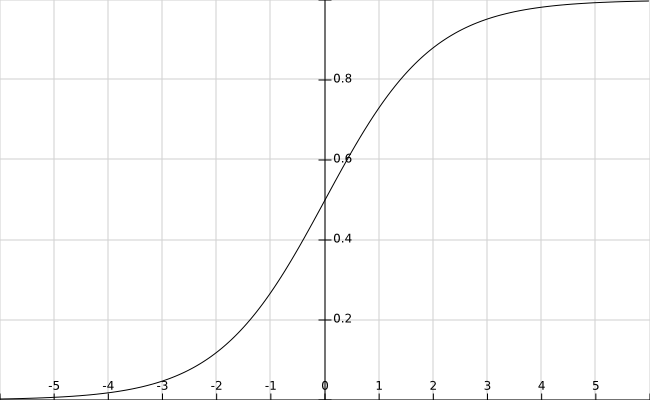
\includegraphics[scale=0.3]{sigmoid}
      \caption{Sigmoidinen funktio}
      \label{pic:sigmoid}
    \end{figure}

    \begin{figure}[h]
      \centering
      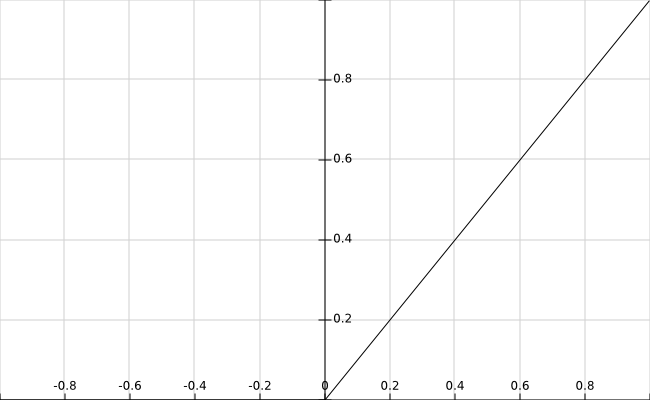
\includegraphics[scale=0.3]{relu}
      \caption{Rectified Linear Unit (ReLU)}
      \label{pic:relu}
    \end{figure}

  %kappaleessa 3 rojanista hyvää juttua \cite{Rojas96}

  %http://neuralnetworksanddeeplearning.com/chap1.html keksi parempi lähde
  % oliko varmasti 50-luvulla?

  \subsection{Keinotekoisten neuroverkkojen rakenne}

  \begin{figure}[h]
    \centering
    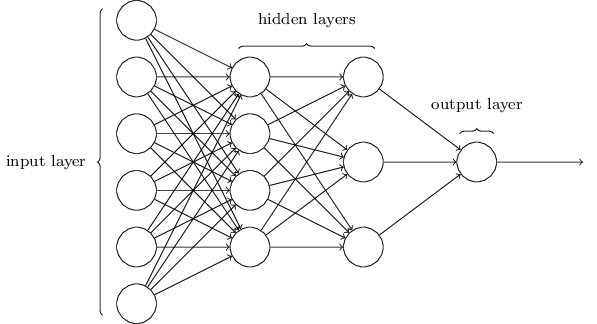
\includegraphics[scale=0.5]{basic-neuralnet}
    \caption{Tyypillinen neuroverkon rakenne, jossa kaksi piilokerrosta \cite{Nielsen-neural}}
    \label{pic:neuralnet}
  \end{figure}

  Yksinkertaisimman verkkorakenteen omaavat eteenpäinsyöttävät neuroverkot muodostetaan kerroksittain niin, että kunkin verkon kerroksen neuronien syötteet ovat niitä edeltävän tason neuroneiden ulostuloarvoja. 
  Yleisimmissä täysin yhdistetyissä (fully connected) neuroverkkokerroksissa jokainen kerroksen neuroni on yhdistetty jokaiseen sitä edeltävän kerroksen neuroniin. Myös muita tapoja yhdistää kerrokset käytetään, kuten esimerkiksi kappaleessa \ref{chap:convolutional-layers} esiteltävissä konvoluutiokerroksissa. 
  
  Neuroverkoissa on aina ainakin syöte- ja ulostulokerros, sekä vaihteleva määrä niiden välissä olevia piilokerroksia. Eteenpäinsyöttävissä neuroverkoissa ei ole silmukoita, eli informaatio kulkee niissä aina vain yhteen suuntaan, syötekerroksesta mahdollisten piilokerrosten kautta kohti ulostulokerrosta, jonka neuroneiden ulostuloarvot ovat neuroverkon laskennan lopputulos. Silmukoita sisältäviä takaisinkytkeytyviä neuroverkkoja on myös olemassa [TODOcite], mutta ne eivät kuulu tämän tutkielman aihepiiriin.

  Kuvassa \ref{pic:neuralnet} vasemmanpuoleisimpana nähdään syötekerros. Esimerkiksi haluttaessa syöttää 64x64 kuva neuroverkolle voidaan syötekerroksena käyttää 64x64 neuronin kerrosta, johon kuvan pikselien väriarvot koodataan.
  % cite???
  Kasvattamalla piilokerroksien sekä kerroksissa olevien neuronien määrää, neuroverkoilla voidaan mallintaa entistä monimutkaisempia funktioita. Vaikka syväoppimista voidaan harjoittaa myös muutoin kuin keinotekoisilla neuroverkoilla, neuroverkkojen tapauksessa termillä viitataan neuroverkkojen piilokerrosten määrään. 

  \section{Neuroverkkojen harjoittaminen}
    \label{chap:neural-training}

  Eteenpäinsyöttävien neuroverkkojen, joissa on yksi piilokerros, on todistettu olevan universaaleja approksimaattoreita \cite{multilayer-feedforward-universal-approximators}. Eteenpäinsyöttävät neuroverkot pystyvät siis approksimoimaan mielivaltaisella tarkkuudella mitä tahansa avaruuden $R^n$ kompakteilla osajoukoilla määriteltyjä jatkuvia funktioita, kunhan tarpeeksi laskentaresursseja on käytettävissä.
  
  %Tulkitsemalla asian asian,  

  %TODO: mieti muotoilua:
  Suurin osa neuroverkkojen ja ylipäätään koneoppimisen sovelluksista hyödyntää mallien harjoittamisessa ohjattua oppimista \cite{nature-lecun15}. Ohjatussa oppimisessa harjoitusaineisto on luokiteltu jollakin perusteella ja harjoittamisvaiheessa pyritään saamaan opetettava malli löytämään näille ennakkoon määritellyille luokille yhteisiä ja harjoitusaineiston ulkopuolisiin syötteisiin yleistettävissä olevia tekijöitä. 
  
  % TODO kysy parinotaatiosta:
  Tyypillinen neuroverkkojen harjoittamiseen käytetty harjoitusaineisto on suuri joukko pareiksi järjestettyjä yksiköitä $ \{(X_i, Z_i)\}_{i=1}^N $ jossa $X_i$ on jokin syötevektori ja $Z_i$ toivottu ulostulovektori tälle syötteelle. Esimerkiksi käsin kirjoitettujen numeroiden kuvista tunnistamista varten tehdyssä harjoitusaineistossa $X_i$ voi olla vektori kuvan pikselien värit määritteleviä arvoja ja $Z_i$ vektori arvoja, jossa vain kuvasta löytyvää numeroa vastaava arvo on asetettu nollasta poikkeavaksi \cite{Nielsen-neural}.

  Laskemalla neuroverkolla harjoitusaineistosta peräisin olevalle syötteelle ulostuloarvo, voidaan saatua ulostuloarvoa verrata harjoitusaineistosta löytyvään toivottuun ulostuloarvoon. Näin neuroverkolle voidaan laskea sen tekemä virhe, ja kun virhe tunnetaan, sitä voidaan pyrkiä pienentämään. 
  Neuroverkkojen harjoittamisen voidaan siis sanoa olevan neuroverkon tekemän virheen minimointia sen approksimoidessa jotakin funktiota.
  
  %TODO: parempi muotoilu, pitäiskö stokastiset hommat mainita jo tässä.
  %todo: cite
  Neuroverkkojen tekemää virhettä mitataan tyypillisesti virhefunktion (error function) avulla. Virhettä halutaan minimoida koko harjoitusaineiston suhteen, joten minimoitava virhefunktio koostetaan useista harjoitusaineiston yksiköistä saatujen virheiden summasta. Usein harjoitusaineistot kuitenkin koostuvat miljoonista yksiköistä jolloin ongelmaksi muodostuu tehokkuus, joten käytännössä yleensä virhe lasketaan vain osalle harjoitusaineistosta.

  %todo lähde
   Hyvin yleisesti käytetään neliöllistä virhefunktiota

  \begin{equation}
    E(x) = \frac{1}{2} \sum_{i=1}^{N} \| y(x_i) - z_i \|^2,
    \label{eq:error-function}
  \end{equation}

  jossa $y(x_i)$ on neuroverkon tuottama tulos jollakin harjoitusaineiston yksikön syötteellä $X_i$, $Z_i$ on harjoitusaineiston perusteella syötteelle $X_i$ toivottu ulostuloarvo, ja $N$ syötteiden määrä. Koska $y(X_i)$ ja $Z_i$ ovat yleensä vektoreita, merkinnällä $\|v\|$ tarkoitetaan erotuksesta muodostuvan vektorin euklidista normia.

  %todo "tuottamaan virheeseen"?
  %todo "menetelmiä minimointiin"?
  %todo lähde
  %todo lasketaanko virhe kerran ja siihen suhteessa kerran painojen derivaatat, vai derivaatta jokaista yksittäistä virhettä kohtaan ja niiden keskiarvo?
  Harjoitusvaiheessa ainoat neuroverkossa muutettavissa olevat parametrit ovat sen neuroneiden syötteiden painotusarvot ja taipumusvakiot. Seuraavaksi esitellään gradienttimenetelmä ja takaisinvirtausalgoritmi, joiden avulla voidaan selvittää, kuinka suuri vaikutus kullakin painotusarvolla ja taipumusvakiolla on koko verkon virheeseen ja muuttaa niitä suuntaan, joka pienentää virhettä.

  % The reason we need this assumption is because what backpropagation actually lets us do is compute the partial derivatives  and  for a single training example. We then recover  and  by averaging over training examples.


  \subsection{Gradienttimenetelmä}
    \label{chap:backprop}

    \begin{figure}[h]
      \centering
      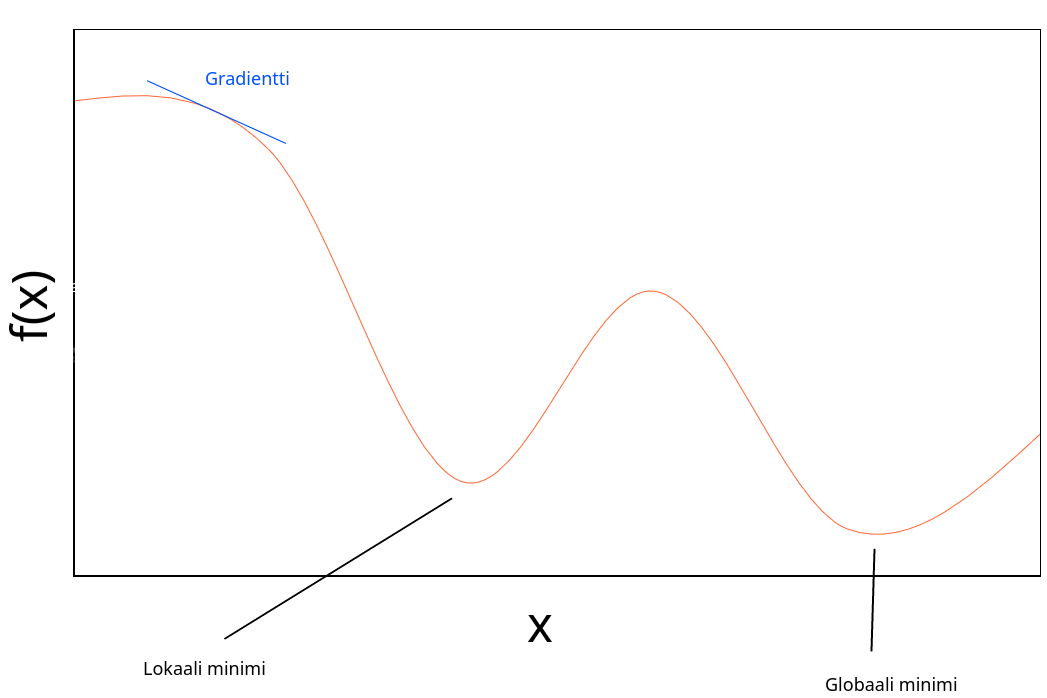
\includegraphics[scale=0.4]{gradient-descent}
      \caption{Gradientti sekä funktion lokaali ja globaali minimi}
      \label{pic:composition}
    \end{figure}

    %TODO muista että takaisinvirtausalgoritmi on yksi tapa toteuttaa gradienttimenetelmää, joten ei "suoriteta gradienttimenetelmää backpropin avulla"
    Gradientti on derivaatan yleistys useamman kuin yhden muuttujan funktioille, joka kertoo mihin suuntaan funktion arvo kasvaa nopeimmin. Gradienttimenetelmällä (gradient descent) tarkoitetaan numeerista menetelmää, jossa kuljetaan iteratiivisesti negatiivisen gradientin suuntaan kunnes gradientti on tarpeeksi pieni. 

    %TODO mieti reluhomman muotoilua
    %TODO kysy assarilta kannattaako Kaavan olla isolla:
    Funktion on oltava derivoituva, jotta sille voidaan muodostaa gradientti, joten myös gradienttimenetelmä edellyttää funktioiden derivoituvuutta. Käytännössä kuitenkin riittää, että aktivaatiofunktiot ovat suurimmilta osin derivoituvia funktioita. 
    Esimerkiksi kappaleessa \ref{chap:artificial-neuron} esitelty ReLU $f(x) = max(0, x)$ ei ole derivoituva kohdassa $x = 0$, mutta sovelluksissa tämä voidaan kiertää vain valitsemalla aktivaatiofunktion derivaataksi tapauksessa $x=0$ jokin kiinteä arvo \cite{Goodfellow-et-al-2016}.
    
    % TODO roskiin?: Neuroverkkojen yhteydessä gradienttimenetelmän käytön helpottamiseksi neuronien aktivaatiofunktioksi valitaan funktioita jotka ovat pääasissa derivoituvia, jolloin myös koko neuroverkon tuottamat arvot ja siten virhefunktio ovat derivoituvia. 

    %TODO: Aktiivisen tutkimuksen muotoilu? Kysy assarilta?
    Vaikka gradienttimenetelmä soveltuukin vain lokaalien minimien etsintään, sen ja sen muunnelmien on huomattu olevan yleensä riittävän toimivia ratkaisuja neuroverkkojen harjoittamiseen \cite{Rumelhart-1986-back-prop}\cite{Goodfellow-et-al-2016}. Toistaiseksi käytännön neuroverkkototeutuksissa on todettu olevan tärkeämpää etsiä parametriavaruudesta sellaisia lokaaleita minimeitä, joissa virhefunktio saa pieniä arvoja, kuin etsiä funktion todellista globaalia minimiä \cite{neural-optimization-goodfellow-2015}. Tämä on kuitenkin vielä aktiivisen tutkimuksen aluetta, josta ei ole varmaa tietoa \cite{Goodfellow-et-al-2016}.

    %todo lähde
    Sen sijaan että virhefunktion gradientin keskiarvo laskettaisiin mahdollisesti miljoonille harjoitusaineiston yksiköille jokaisella harjoituskierroksella, yleensä käytetään stokastista gradienttimenetelmää, jossa gradientin keskiarvo muodostetaan vain osasta harjoitusaineistoa. 
    %TODO: Stokastisen gradienttimenetelmän on todettu tuottavan hyviä tuloksia.

    %Virhefunktion arvon laskeminen jokaiselle syötteelle ja keskiarvon ottaminen ja tämän perusteella takaisinvirtausalgoritmin suorittaminen olisi erittäin raskasta, kun syötteitä voi olla miljoonia kappaleita. Tämän takia käytetään yleensä stokastista gradienttimenetelmää, jossa virhefunktion keskiarvo lasketaan kaikkien syötteiden sijaan joukolle satunnaisesti valittuja syötteitä, ja suoritetaan seuraavaksi esiteltävä takaisinvirtausalgoritmi tämän tuloksen perusteella.


  \subsection{Takaisinvirtausalgoritmi}
    Takaisinvirtausalgoritmilla viitataan kaksivaiheiseen neuroverkkojen opetusprosessiin. Eteenpäinvirtaukseksi kutsutaan ensimmäistä vaihetta, jossa neuroverkon virhe lasketaan jollekkin harjoitusaineiston osajoukolle aikaisemmin esitellyllä tavalla. Taaksepäinvirtaukseksi, josta algoritmi on saanut nimensä, kutsutaan virheen kuljettamista verkossa ulostulokerroksesta takaisin kohti syötekerrosta virhefunktion osittaisderivaattojen selvittämiseksi verkon painotusarvojen ja taipumusvakioiden suhteen. Kun virhefunktion osittaisderivaatat painotusarvojen ja taipumusvakioiden suhteen tunnetaan, voidaan niistä muodostaa gradientti ja soveltaa gradienttimenetelmää virheen minimoimiseksi.

    \begin{figure}[h]
      \centering
      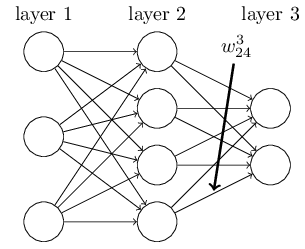
\includegraphics[scale=0.4]{neuron-notation}
      \caption{Painotuksiin viittaamiseen käytetty notaatio \cite{Nielsen-neural}.}
      \label{pic:chain-rule}
    \end{figure}

    Algoritmin käsittelyn helpottamiseksi käytetään verkon osiin viittaamiseen alan kirjallisuudessa yleisesti käytettyä notaatiota likimain vastaavia merkintätapoja \cite{Nielsen-neural}\cite{Rojas96}. Kerroksessa $l$ olevan $i$:nnen neuronin ulostuloarvosta käytetään merkintää $out_i^l$, neuronin painotettujen syötteiden summasta merkintää $net_i^l$, kerroksessa $l-1$ olevan $i$:nnen neuronin ja kerroksessa $l$ olevan $j$:nnen neuronin välillä olevasta painotuksesta merkintää $w_{ji}^l$, ja koko verkon virheestä merkintää $E_{koko}$. Käydään seuraavaksi läpi, kuinka virhefunktion derivaatta yksittäisen painotusarvon suhteen selvitetään ensin ulostulokerroksessa, ja tämän jälkeen muissa kerroksissa.

    %n $l-1$ ja $l$ $i$:nnen ja $j$:nnen neuroneiden välillä olevasta painotuksesta merkintää $w_ji$

    %Kerroksissa $l-1$ ja $l$ olevien neuronien $n_i^{l-1}$ ja $n_j^{l}$ välillä olevan verkon painon $w_{ji}^l$

    %TODO kuva jostain mihin voi viitata
    \begin{figure}[h]
      \centering
      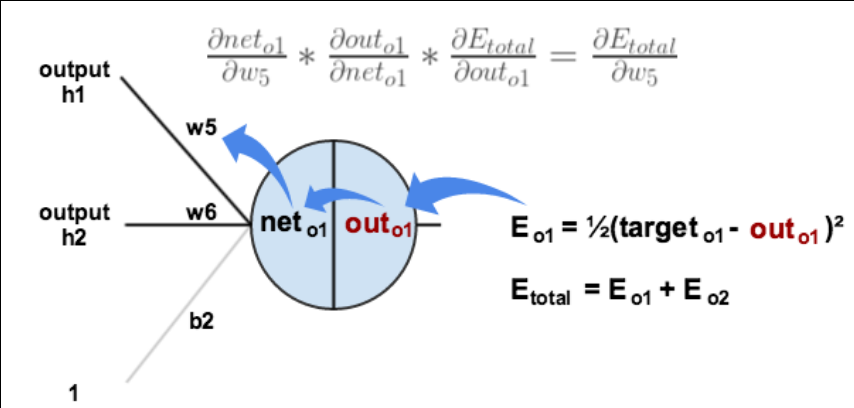
\includegraphics[scale=0.4]{chain-rule}
      \caption{Virhefunktion derivaatta syötteen painotuksen suhteen}
      \label{pic:chain-rule}
    \end{figure}

    Virhefunktion derivaatta painotuksen suhteen voidaan laskea derivaatan ketjusäännön avulla

    $$ \frac{\partial E_{koko}}{\partial w_{ji}^l} = \frac{\partial E_{koko}}{\partial out_j^{l}} \cdot \frac{\partial out_j^{l}}{\partial net_j^{l}} \cdot \frac{\partial net_j^{l}}{\partial w_{ji}^l}$$

    \noindent Kuvan \ref{pic:chain-rule} mukaisesti. Käydään järjestyksessä läpi kuinka yhtälön oikean puolen kolme termiä selvitetään. 
    
    Yhtälön oikean puolen ensimmäinen termi ulostulokerroksen tapauksessa saadaan ottamalla Kaavan \ref{eq:error-function} mukaisesta virhefunktiosta osittaisderivaatta $out_j^{L}$ suhteen, jossa $L$ on ulostulokerros, jolloin summan muut termit katoavat ja jäljelle jää 

    $$\frac{\partial E_{koko}}{\partial out_j^{L}} = 2 \cdot \frac{1}{2} (out_{j}^{L} - z_j)^{2-1} = out_{j}^{L} - z_j.$$
    
    \noindent Toinen termi on käsiteltävän neuronin aktivaatiofunktion derivaatta
    $$\frac{\partial out_j^{l}}{\partial net_j^{l}} = f'.$$

    \noindent Kolmannen termin kohdalla huomataan otettaessa neuronin summausfunktiosta osittaisderivaatta jonkin sen painotuksen suhteen, muut termit ovat vakioita, joiden derivaatta on 0, $w_{ji}^l$ derivaatta itsensä suhteen on 1, jolloin jäljelle jää

    $$ \frac{\partial net_j^{l}}{\partial w_{ji}^l} = 1 \cdot out_i^{l-1} = out_i^{l-1}. $$
    
    Muiden kerroksien kohdalla jälkimmäiset kaksi termiä kolmesta voidaan muodostaa samalla tavalla, mutta ensimmäisen termin laskeminen on monimutkaisempaa, sillä on otettava huomioon, että muissa kuin ulostulokerroksessa neuronien ulostuloarvot vaikuttavat niitä seuraavien kerrosten ulostuloarvoihin ja siten virheisiin. Tällöin 

    $$ \frac{\partial E_{koko}}{\partial out_j^l} = \sum_{k=1}^{N} \frac{\partial E_{k}^{l+1}}{\partial out_j^l},$$

    jossa $ E_{k}^{l+1} $ viittaa niistä $l+1$ kerroksen neuroneista, jotka saavat yhtenä syötteistään arvon $out_j^l$, koostuvan osajoukon $k$:nnen neuronin ulostuloarvon osuuteen koko verkon virheestä. Koska algoritmia suoritetaan ulostulokerroksesta syötekerrokseen päin, summan termien selvittämisessä voidaan hyödyntää aikaisemmissa kerroksissa laskettuja välituloksia ja ketjusääntöä. Saadaan

    $$ \frac{\partial E_{k}^{l+1}}{\partial out_j^l} = \frac{\partial E_{k}^{l+1}}{\partial net_k^{l+1}} \cdot \frac{\partial net_k^{l+1}}{\partial out_j^l}, $$

    \noindent joista yksinkertaisempi jälkimmäinen termi
    
    $$ \frac{\partial net_k^{l+1}}{\partial out_j^l} = w_{kj}^{l+1}, $$

    \noindent ja ensimmäinen termi
    $$ \frac{\partial E_{k}^{l+1}}{\partial net_k^{l+1}} = \frac{\partial E_{k}^{l+1}}{\partial out_k^{l+1}} \cdot \frac{\partial out_k^{l+1}}{\partial net_k^{l+1}}, $$

    \noindent jonka ensimmäinen termi on jonkin syötteenään $out_j^l$ ottavan neuronin $n$ ulostuloarvon $out_k^{l+1}$ virheen vaikutus kokonaisvirheeseen, joka on valmiiksi laskettu sitä neuronia käsiteltäessä, ja toinen termi neuronin $n$ aktivaatiofunktion $f$ derivaatta $f'$. Nähtiin siis syötekerrosta lähempien kerrosten virheiden laskentaan tarvittavan ensin ulostulokerrosta lähempien kerrosten neuroneiden virheet, joten virheen voidaan ajatella virtaavan ulostulokerroksesta kohti syötekerrosta.
    % ^ todo mieti vikan lauseen muotoilua.
    % todo mainitse biasista
  \subsection{Oppimistahti ja aloituspainot}
  Kun 

  $$\frac{\partial E_{koko}}{\partial w_{ji}^{l}}$$
  
  %TODO kai tähän voisi jonkun perus lähteen hakea, tai ehkä gradienttimenetelmäkappaleessa riittää?
  \noindent tiedetään, virhettä pyritään pienentämään muuttamalla painotusta jonkin oppimistahdin (learning rate) $-\eta$ mukaisesti. Virhefunktiolle laskettu gradientti itsessään kertoo vain suunnan infinitesimaalisella alueella johon siirtymällä virhefunktio kasvaa eniten, mutta ei optimaalista askeleen kokoa. Negatiivisen oppimistahdin avulla siirrytään gradientin osoittamaa virhefunktion suurimman kasvun suuntaa vastakkaiseen suuntaan

  
  $$ w_{ji}^{l} = w_{ji}^{l} - \eta \cdot \frac{\partial E_{koko}}{\partial w_{ji}^{l}}, $$

  %TODO kysy viittaustavasta jossa pisteen ulkpuolella. muutenki paska muotoilu
  \noindent joka pienentää neuroverkon virhettä, mikäli oppimistahti on riittävän pieni. Oppimistahdin valintaan ja muuttamiseen harjoittamisen aikana löytyy lukuisia heuristisia menetelmiä, joista yleisimpänä jonkin pienen arvon valitseminen aluksi, ja sen pienentäminen oppimisen alkaessa hidastumaan harjoittamisen aikana. \cite{Goodfellow-et-al-2016}\cite{KSHimagenet2012}

  Verkon aloituspainojen valinnassa olennaisinta on, että kaikki painotukset eivät ole samoja, koska silloin virhefunktion gradientti on näille painotuksille aina sama, eivätkä neuronit pysty erikoistumaan. Yleisin tapa painojen alustamiseen on valita niille satunnaisia pieniä arvoja jostakin satunnaisjakaumasta. Taipumusvakioiden aloitusarvot valitaan usein heuristisesti. \cite{Goodfellow-et-al-2016}


  %alkup. backprop paperissa on symmetry breakingista
  %...
  \subsection{Esimerkki harjoittamisesta}

  Lasketaan ensin neuroverkon antama tulos esimerkkisyötteelle satunnaisesti alustetuin painotuksin ja selvitetään sen jälkeen takaisinvirtausalgoritmin avulla yhdelle verkon painotukselle uusi arvo, joka vähentää verkon tekemää virhettä esimerkin harjoitusaineiston yksiköllä. Esimerkin neuroverkko on eteenpäinsyöttävä, siinä ei ole taipumusvakioita, ja siinä on kolme kerrosta: syötekerros, täysin yhdistetty piilokerros, sekä täysin yhdistetty ulostulokerros. Kussakin kerroksessa on 2 neuronia. Oppimistahtina käytetään mielivaltaisesti valittua arvoa $\eta = 0.5$.
  %TODO: keksi onko eq:sigmoid-func todella lauseke vai mikä?
   Aktivaatiofunktiona käytetään Lausekkeessa \ref{eq:sigmoid-func} esiteltyä sigmoidista funktiota $\sigma (x)$.

    \begin{figure}[h]
    \centering
    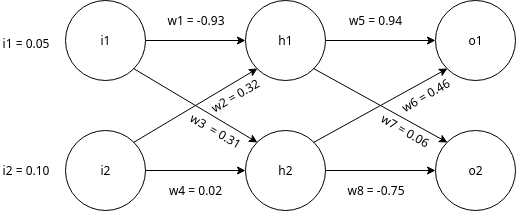
\includegraphics[scale=0.6]{draw-io-backprop-example}
    \caption{Esimerkin neuroverkon syötteet ja painotukset}
    \label{pic:backprop-example}
    \end{figure}

  Lasketaan ensin verkon tuottamat ulostuloarvot syötteillä $i_1 = 0,05$ ja $i_2 = 0,10$ sekä väliltä $[-1, 1]$ arvotuilla painotuksilla $w_1...w_8$. Piilokerroksen neuroneiden syötteiden summaus tehdään kappaleessa \ref{chap:artificial-neuron} esitetyn kaavan $\Sigma x_i w_i$ mukaisesti
  
  $$h_{1}^{net} = w_1 \cdot i_1 + w_2 \cdot i_2 \approx -0.0145$$
  % $$h_{1}syöte = -0,93 * 0,05 + 0,32 * 0,10 = -0,0145$$
  $$h_{2}^{net} = w_3 \cdot i_1 + w_4 \cdot i_2 \approx 0.0175.$$
  % $$h_{2}^{in} = 0,31 * 0,05 + 0,02 * 0,10 = 0,0175$$

  Syöttämällä nämä arvot sigmoidiseen aktivaatiofunktioon saadaan
  $$h_{1}^{out} = \sigma(h_{1}^{in}) \approx 0.496$$
  $$h_{2}^{out} = \sigma(h_{2}^{in}) \approx 0.504.$$

  Toistaen vastaavat vaiheet ulostulokerrokselle käyttäen piilokerroksen ulostuloarvoja syötteenä saadaan:
  $$o_{1}^{net}= w_5 \cdot h_1 + w_6 \cdot h_2 \approx 0.628$$
  %$$o_{1}syöte = 0,94 * 0,496 + 0,32 * 0,504 \approx 0,628$$
  $$o_{2}^{net}= w_7 \cdot h_1 + w_8 \cdot h_2 \approx -0.348$$
  %$$o_{2}syöte = 0,06 * 0,496 + (-0,75) * 0,504 \approx -0,348$$

  $$o_{1}^{out} = \sigma(o_{1}^{net}) \approx 0.652$$
  $$o_{2}^{out} = \sigma(o_{2}^{net}) \approx 0.414.$$

  %Kun harjoitusaineistoksi valitaan arvot $o_1harjoitus = 0.01$ ja $o_2harjoitus = 0.99$ saadaan kaavan \ref{eq:error-function} mukaisesta virhefunktiosta $E(x) = \frac{1}{2} \sum_{i=1}^{N} \| y(x_i)-a(x_i) \|^2$ arvoksi
  Kun harjoitusaineistoksi valitaan arvot $z_{1}^{out} = 0.01$ ja $z_{2}^{out} = 0.99$ saadaan kaavan \ref{eq:error-function} virhefunktiosta 

  
  $$ \frac{1}{2} \cdot ( (o_{1}^{out} - z_1^{out})^2 + (o_{2}^{out} - z_2^{out})^2 ) \approx 0.372. $$

  % $$ 0,5 * ( (0,652 - 0,01)^2 + (0,414 - 0,99)^2 ) = 0,372. $$

  Lasketaan painon $w_5$ vaikutus virheeseen. $E_{koko}$ koostuu ulostulokerroksen neuroneiden tekemien virheiden summista, joten kun se derivoidaan tietyn neuronin ulostulon suhteen, muiden neuroneiden virheiden termit putoavat pois. Jäljelle jää 
  
  $$ \frac{\partial E_{koko}}{\partial o_{1}^{out}} = 2 \cdot \frac{1}{2} (o_{1}^{out} - z_1^{out})^{2-1} \cdot 1 = o_{1}^{out} - z_1^{out} = 0.651$$

  Aktivaatiofunktion $\sigma (x)$ derivaatta on $\sigma'(x) = \sigma(x) \cdot (1 - \sigma(x))$.
  Koska 
  
  $$ o_{1}^{out} = \sigma(o_1^{net}) $$
  
  niin

  %$$ \frac{\partial o_{1}^{out}}{\partial o_1^{summa}} = o_{1}^{out}(1 - o_{1}^{out}) = 0.652(1 - 0.652) \approx 0.227.$$
  $$ \frac{\partial o_{1}^{out}}{\partial o_1^{net}} = o_{1}^{out} \cdot (1 - o_{1}^{out}) \approx 0.227.$$

  $$ o_1^{net} = w5 \cdot h_{1}^{out} + w_6 \cdot h_{2}^{out} $$
  
  joten viimeinen tarvittava osa 
  $$ \frac{\partial o_1^{net}}{\partial w_5} = 1 \cdot h_{1}^{out} + w_5 \cdot 0 + 0 = out_{h1} $$ 

  joten 
  
  $$\frac{\partial E_{koko}}{\partial w_5} = 0.651 \cdot 0.227 \cdot 0.496 \approx 0.073. $$

   Korjaamme nyt $w_5$ virhettä asettamalla sen uudeksi arvoksi

  $$w_{5}^+ = w_5 - \eta \cdot \frac{\partial E_{koko}}{\partial w_5} = 0.9035.$$


  % syötteet: 0.05, 0.10
  % painot: -0.93 0.31 0.32 0.02 0.94 0.06 0.46 -0.75
  % toivotut ulostulot 0.01 0.99



  \subsection{Ylisovitus ja sen ratkaiseminen}

  %Koneoppimisessa haaste ylisovitus
  Suuri haaste neuroverkkojen harjoittamisessa on ylisovitus (overfitting), jossa neuroverkon harjoittamisen jälkeen neuroverkko saa harjoitusaineistosta valituille syötteille pieniä arvoja virhefunktiosta, mutta uuden aineiston kanssa virhefunktio tuottaa suuria arvoja \cite{Nielsen-neural}. Tällöin neuroverkon oppima approksimaatio vastaa harjoitusaineistoa liian tarkkaan, eikä pysty yleistämään harjoitusaineistosta löytyviä ominaisuuksia aineiston ulkopuolisille syötteille. Ylisovittamisen välttäminen on sitä vaikeampaa, mitä enemmän verkossa on opittavia parametreja, mistä johtuen sen välttämiseksi kehitetyt menetelmät ovat muuttuneet tärkeämmiksi modernien neuroverkkojen kasvaessa yhä suuremmiksi. 
  
  %todo liian lyhyt
  Neuroniyksikköjen pudotus (dropout) on menetelmä, jossa harjoitusvaiheessa yksittäisiä neuroneita poistetaan satunnaisesti käytöstä, jolloin yksittäiset neuronit naapureineen eivät erikoistu tiettyihin aineiston ominaisuuksiin liian tarkasti \cite{dropout-srivastava}.

  %todo liian lyhyt
  L2 regularisaatiossa neuroverkon virheeseen lisätään arvo $\lambda \sum_{i=1}^N$ jossa $\lambda$ on regularisaatioparametri ja $N$ on painojen määrä. Tällä lisäyksellä neuroverkko saadaan priorisoimaan pieniä painotusarvoja \cite{ng2004feature}.
  
  %todo poista koko kappale tai lisää viite
  Ylisovitusta voidaan vähentää myös laajentamalla harjoitusaineistoa. Esimerkiksi kuvien tunnistuksessa harjoitusaineiston kokoa on kasvatettu kääntämällä ja siirtämällä kuvia, ottamalla kuvista osakuvia ja skaalaamalla niitä suuremmaksi ja pienemmäksi, sekä lisäämällä kuviin satunnaista kohinaa. Puheentunnistuksessa harjoitusaineistoon on lisätty kohinaa ja erilaisia muita ylimääräisiä ääniä.

  
  \section{Konvolutionaalisten neuroverkkojen rakenne}
  %TODO mainitse miten backpropagation toimii CNN:ien kanssa

    %Tässä kappaleessa käydään läpi Michael A. Nielsen, Neural Networks and Deep Learning \cite{Nielsen-neural} kirjaan pohjautuen perusteet konvolutionaalisten neuroverkkojen rakenteesta. 
    Konvolutionaalisten neuroverkkojen rakenne eroaa tavanomaisista täysin yhdistetyistä neuroverkoista konvoluutio- ja kokoamiskerroksien (pooling layer), kerrosten mahdollisen rinnakkaisuuden, sekä piirrekuvausten jaettujen painojen kautta \cite{Lecun-et-al-1928-convnets}.   
    

    %(TODO:lisää kuvia ja selitystä ytimestä, kuten esitelmähommassa puhuttiin)
    % esim värittämällä kernelin/feature mapin painotukset nähdään millaisia featureja se etsii
    \subsection{Konvoluutiokerrokset}
    \label{chap:convolutional-layers}

    \begin{figure}[h]
      \centering
      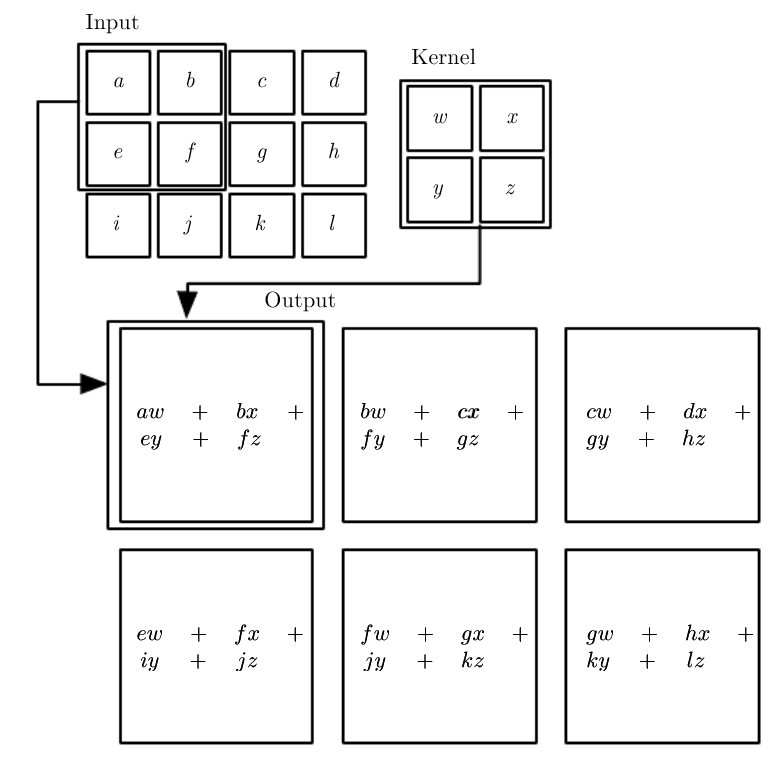
\includegraphics[scale=0.4]{convolution}
      \caption{Konvoluutiokerrosten syötteiden valinta ja ulostulojen muodostuminen \cite{Goodfellow-et-al-2016}}
      \label{pic:convolution}
    \end{figure}

    Konvolutionaalisten neuroverkkojen nimi juontaa juurensa matemaattiseen konvoluutioon. Konvoluutiokerrosten neuroneiden syötteet $a_{x,y}$ painotuksineen $w_{x,y}$ voidaan esittää matemaattisesti esimerkiksi 5x5 kokoiselle paikalliselle vastaanottavalle kentälle (local receptive field) muodossa

    % TODO: kuuluuko loppuun pilkku?
    $$ \sum_{l=0}^{4}\sum_{m=0}^{4} w_{l,m}a_{j+l,k+m},$$
    
    \noindent joka on käytännössä diskreetti konvoluutio, jossa painotukset ovat konvoluution ydin (kernel).

    Konvoluution voidaan ajatella olevan liukuva ikkuna, joka rajoittaa neuronit saamaan kuvan \ref{pic:convolution} mukaisesti syötteenään vain osan syötekerroksensa ulostuloista, täysin yhdistetyistä neuroverkkokerroksista poiketen. Tämä rajoittuneisuus mahdollistaa neuroneiden erikoistumisen johonkin osa-alueeseen syötteissään, joka on erityisen hyödyllistä haluttaessa käyttää neuroverkkoja syötteiden tutkintaan joissa ilmenee paikallisuutta. Esimerkiksi kuvat ovat erittäin paikallistuneita, pikselien etäisyys toisistaan korreloi vahvasti sen kanssa, liittyykö niiden sisältö toisiinsa.

    Kuvasta \ref{pic:convolution} ilmenee myös toinen yleinen konvoluutiokerrosten piirre: mikäli tehdään vain konvoluutioita joissa ydin mahtuu kokonaan syötekuvaan, konvoluutiokerroksella on vähemmän ulostuloja kuin sisääntuloja. Kuvan tapauksessa nähdään syötematriisin ollessa 3x4, ja ytimen 2x2 kokoinen, ulostulomatriisin kooksi tulee 2x3. Tällä tavalla konvoluutio mahdollistaa myös sen, että konvoluutioverkot voivat ottaa vastaan vaihtelevan kokoisia syötteitä.

    \subsection{Piirrekuvaukset ja jaetut painot}
    % TODO: ei yhtään viitettä
  TODO: lisää kuvia yms. siitä mitä ydin on jne.
    \begin{figure}[h]
      \centering
      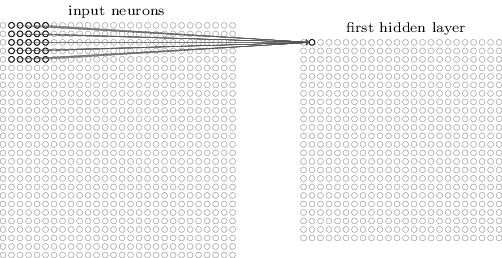
\includegraphics[scale=0.5]{local-receptive}
      \caption{Piirrekuvaus \cite{Nielsen-neural}}
      \label{pic:local-receptive}
    \end{figure}

  % TODO selitä lisää miten yhteiset painot toimivat
    Konvoluutiokerroksia on yleensä useita rinnakkain, ja konvoluutiokerrosten neuronit jakavat samassa kerroksessa olevien neuroneiden kesken yhteiset painot (shared weights). Kerroksien yhteiset painot mahdollistavat sen, että kukin kerros oppii tunnistamaan translationaalisesti invariantteja ominaisuuksia syötteistään, ja yksittäisen neuronin voidaan ajatella kertovan löytyykö sen saamien syötteiden alueelta tätä ominaisuutta. Esimerkiksi kuvien tapauksessa piirrekuvaus joka löytää kuvasta suoria viivoja saattaa olla hyödyllinen, sillä suoria viivoja voi ilmetä useassa eri paikassa kuvassa, ja toisaalta korkeammalla abstraktiotasolla kuvassa esiintyvä objekti on edelleen sama objekti, vaikka sitä olisi siirretty muutamia pikseleitä johonkin suuntaan.

    \subsection{Kokoaminen ja tehokkuus}
    Usein konvoluutioverkoissa käytetään konvoluutiokerroksien jälkeen kokoamiskerroksia, jotka tekevät yhteenvedon jostakin edeltävästä neuroverkkokerroksen alueesta. 
    % todo max poolauksesta käytännön esimerkki kuvineen
    Esimerkiksi hyvin yleisen maksimikokoamiskerroksen (max-pooling) neuronit antavat ulostulokseen syöteneuroniensa ulostuloista suurimman.
    %todo viitteet viitteet viitteet

    Yhdessä kokoamiskerrokset ja jaetut painotukset vähentävät merkittävästi konvolutionaalisten neuroverkkojen harjoitettavien parametrien määrää verrattuna neuroverkkoihin, joissa on vain täysin yhdistettyjä kerroksia. Tällä voidaan nopeuttaa harjoittamista ja lisätä suorituskykyä.

    \subsection{Täysin yhdistetyt kerrokset}
    %TODO: miksi kerrokset haluttaisiin litistää takaisin yhteen?
    Konvoluutiokerrosten kohdalla konvolutionaaliset neuroverkot haarautuvat yleensä rinnakkaisiin kerroksiin. Sijoittamalla verkon viimeiseksi kerrokseksi täysin yhdistetyn kerroksen nämä rinnakkaiset kerrokset voidaan litistää (flattening) takaisin yhteen.

  \section{Konvolutionaaliset neuroverkot käytännössä}


    %\subsection{Kirjastot}
    %Johonkin saisi ehkä pari kappaletta tekstiä (konvolutionaalisten) neuroverkkojen luomista helpottavista kirjastoista yms. kuten TensorFlow.
    
  %\subsection{Verkon toiminnan visualisointi}
  %... \cite{visualizing-convolutional}

  \subsection{Kuvien luokittelu}
    Konvoluutioverkkoja on käytetty erityisen onnistuneesti kuvien sisällön luokitteluun.

    Monille kuvia tunnistaville neuroverkoille yhteinen piirre on, että ulostulokerroksessa on yksi neuroni jokaista tunnistettavaa objektiluokkaa kohden, ja neuronin arvo kertoo kuinka todennäköisesti kyseisen luokan objekti löytyy kuvasta. TODO: Softmax





    % \subsection{ImageNet kilpailu}
    %   ...

    % ...
    TODO: Imagenet kilpailun kuvailu? Pitäisikö olla oma kokonainen section kuvien luokittelulle ja sen subsectionina imagenet ja CNN:ien toiminnan visualisointi. Esimerkkikuvia imagenet aineistosta?

    TODO taulukko imagenetissa tunnistusprosentin paranemisesta

    \begin{figure}[h]
    \centering
    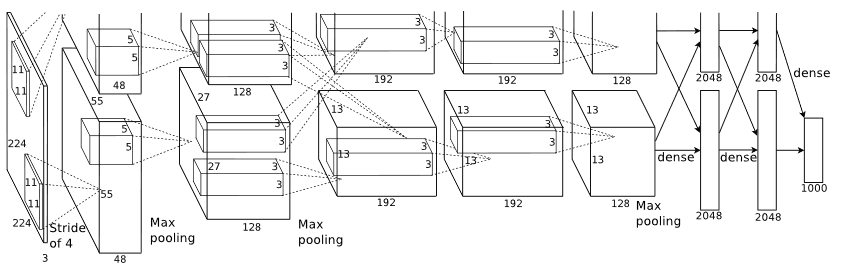
\includegraphics[scale=0.4]{imagenet}
    \caption{ILSVRC-2012 kilpailun voittaneen neuroverkon rakenne \cite{KSHimagenet2012}}
    \label{pic:hsk-neuralnet}
    \end{figure}

    % TODO https://arxiv.org/pdf/1710.05941.pdf mainitaan että ReLU oli tosi tärkee tälle 2012 setille
    Vuonna 2012 ImageNet kuvantunnistuskilpailun voittaneessa Krizhevsky, Sutskever ja Hintonin (myöhemmin KSH) konvolutionaalisessa neuroverkossa on 7 piilokerrosta, joista 5 ensimmäistä ovat konvoluutiokerroksia, ja 2 viimeistä kerrosta täysin yhdistettyjä kerroksia. KSH:ssa on 1000 neuronin ulostulokerros joka vastaa sen tunnistamaa tuhatta erilaista kuvaluokkaa.
    
    ImageNet kuvamateriaalissa on vaihtelevan kokoisia kuvia, mutta KSH:n luomassa neuroverkon syötekerros oli 3x224x224 neuronin kokoinen. KSH:n ratkaisu syötteen sopivaksi saamiseksi oli skaalata lähdekuvat ensin 256x256 pikselin kokoon, ja tämän jälkeen ottaa kuvista 224x224 osakuvia satunnaisista sijainneista lähdekuvasta, näin laajentaen harjoitusdataa ja vähentäen ylisovitusta.
    
    KSH:n verkossa aktivaatiofunktiona toimi viimeaikoina hyväksi havaittu $R(z) = max(0, z)$ muotoinen Rectified Linear Unitiksi (ReLU) kutsuttu funktio \cite{KSHimagenet2012}.

  imagenet klassifikation \cite{KSHimagenet2012} learning rateksi valittiin ensin 0.01, ja sitä pienennettiin jakamalla sen arvo ymmenellä aina kun oppimisen huomattiin loppuneen.

  %\subsection{Deep dream}
  %Samanlainen toteutustapa kuin takaisinvirtausalgoritmissa, paitsi painotusarvot pysyvät kiinteinä ja muutetaankin syötettä.


\section{Yhteenveto} 

Kappale siitä, että sitä ei vielä täysin ymmärretä, miksi neuroverkot oppivat niin hyvin. Täs vois mainita \cite{neural-optimization-goodfellow-2015} :sta siitä abstraktissa mainitusta jutusta et pitkään pelättiin et neuroverkkojen treenaus ois super vaikeeta

Aloitettiin käymällä läpi kaikille neuroverkoille yleisiä piirteitä, kuten yksittäisen neuronin rakennetta ja sitä, miten yksittäisistä neuroneista muodostetaan eteenpäinsyöttävä neuroverkko. Seuraavaksi esiteltiin kuinka neuroverkkoja voidaan harjoittaa harjoitusaineiston perusteella takaisinvirtausalgoritmin ja gradienttimenetelmän avulla. Lopuksi käsiteltiin konvolutionaalisten neuroverkkojen eroavaisuuksia muista neuroverkoista ja esiteltiin käytännön esimerkki konvolutionaalisesta neuroverkosta.

Käsittelemättä jäi miten aktivaatiofunktioita, hyperparametrejä yms. valitaan järkevästi/hyvin (myös koska niistä ei juuri ymmärretä ja hyvin vaikea tehtävä). Muista neuroverkkorakenteista kuin eteenpäinsyöttävistä konvoluutioverkoista ei kerrottu, esim RNN, muut jotku poolaukset, jne






  % ------------------------------ References ------------------------------
  %
  % bibtex is used to generate the bibliography. The babplain style
  % will generate numeric references (e.g. [1]) appropriate for theoretical
  % computer science. If you need alphanumeric references (e.g [Tur90]), use
  %
  % \bibliographystyle{babalpha-lf}
  %
  % instead.

  %\nocite{*}
  \bibliographystyle{babplain-fl}
  \bibliography{references}


  % --- Appendices ---

  % uncomment the following

  % \newpage
  % \appendix
  %
  % \section{Esimerkkiliite}

  \end{document}
